\chapter{Results and Discussion}
The results presented here concern the solution of the adiabatic equation. In order to obtain potential curves I solve Eq. \eqref{adiabatic} using a local function expansion such as the basis splines, thus determining the adiabatic potential curves Uν(R)
164
and the set of orthonormal channel functions Φν(R; φ, θ) that depend parametrically on R. In order to reach the assymptotic regime 
I have calculated The adiabatic equation \eqref{adiabatic} has been solved 
\begin{table}[h!]
	\centering
	\begin{tabular}{||c c c c c c||} 
		\hline
		$N_{\theta}$ & $\lambda_{0 0}$ & $\lambda_{1 3}$ & $\lambda_{2 6}$ & array(s) & dsygvd(s)
		\\ [0.5ex] 
		\hline\hline
		5	   & 0.000 000 000 0214   & 32.000 000 071 3015 & 60.000 002 031 0135 & 0.66 & 0.00  \\
		10     & -0.000 000 000 0417  & 32.000 000 000 1003 & 60.000 000 000 2154  & 4.58 & 0.00 \\
		15 & 0.000 000 000 0007 & 32.000 000 000 1309 & 59.999 999 999 8871& 12.32& 0.02 \\  [1ex] 
		\hline
	\end{tabular}
	\caption{Numerically calculated eigenvalues}
	\label{table:2}
\end{table}

\begin{figure}
	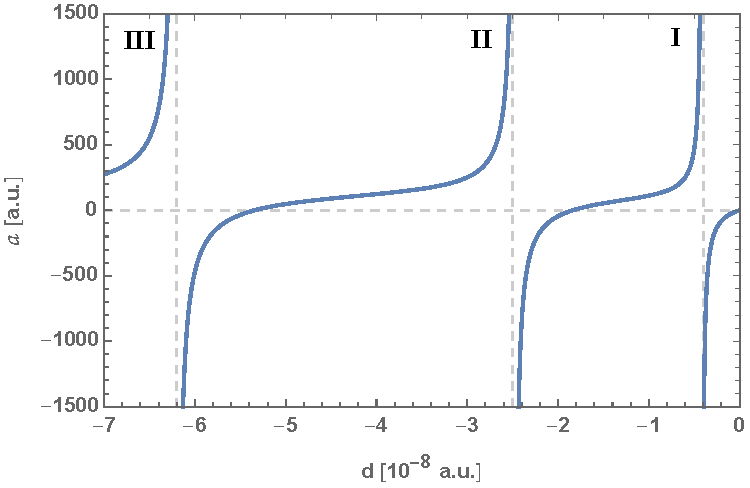
\includegraphics[width=\linewidth]{scatteringlength.pdf}
	\caption{The two-body scattering length as a function of the potential depth $d$. Three poles can be recognized in the figure, labelled $\mathrm{I},\mathrm{II},\mathrm{III}$. At each pole a new two-body bound state is formed. The first bound state is formed as $a$ passes through $\mathrm{I}$, followed by a second a two-body bound state is formed. At each pole a new two-body bound state is formed, so when $\abs{d}$ is increased so that $a$ passes through $\mathrm{II}$ a second two-body bound state is formed, while a third state is formed as $a$ passes through $\mathrm{III}$.}
	\label{fig:3}
\end{figure}

\begin{figure}
	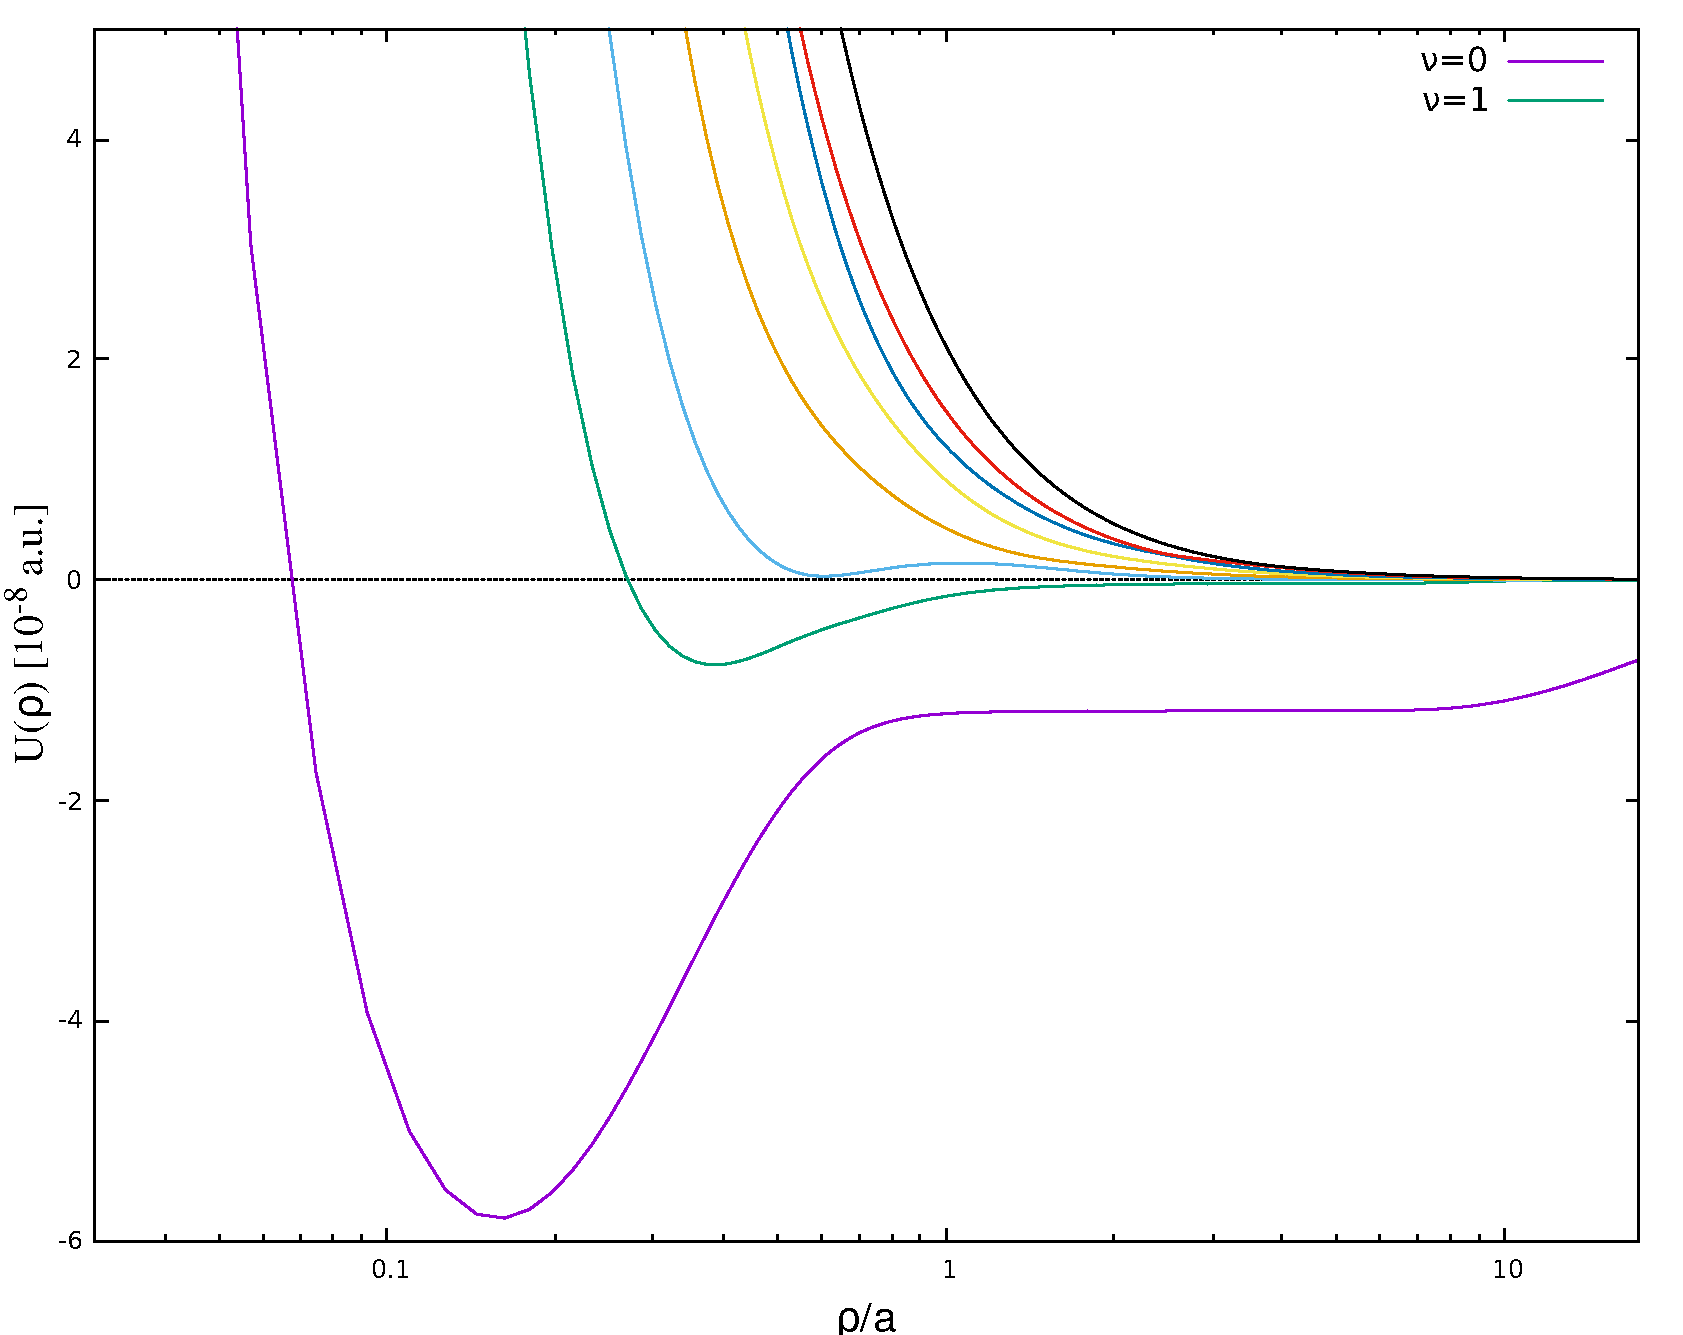
\includegraphics[width=\linewidth]{adiabatic.pdf}
	\caption{Adiabatic potential curves $U_{\nu}$ as a function of the hyperradius $\rho$ for $a=228 $ .}
	\label{fig:3}
\end{figure}

\begin{figure}
	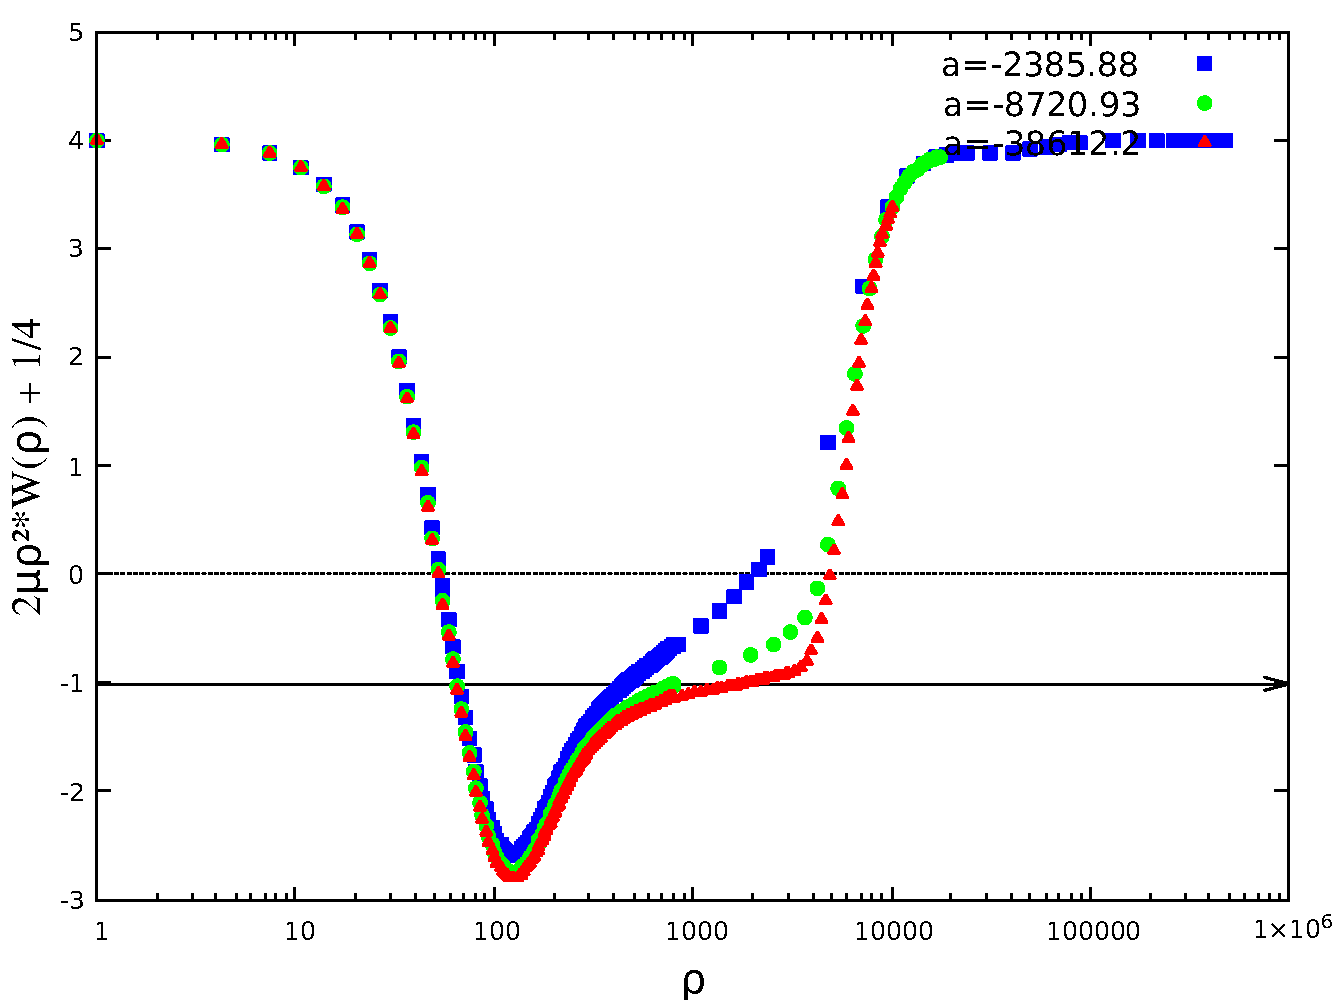
\includegraphics[width=\linewidth]{negativ_a.pdf}
	\caption{..}
	\label{fig:5}
\end{figure}

\begin{figure}
	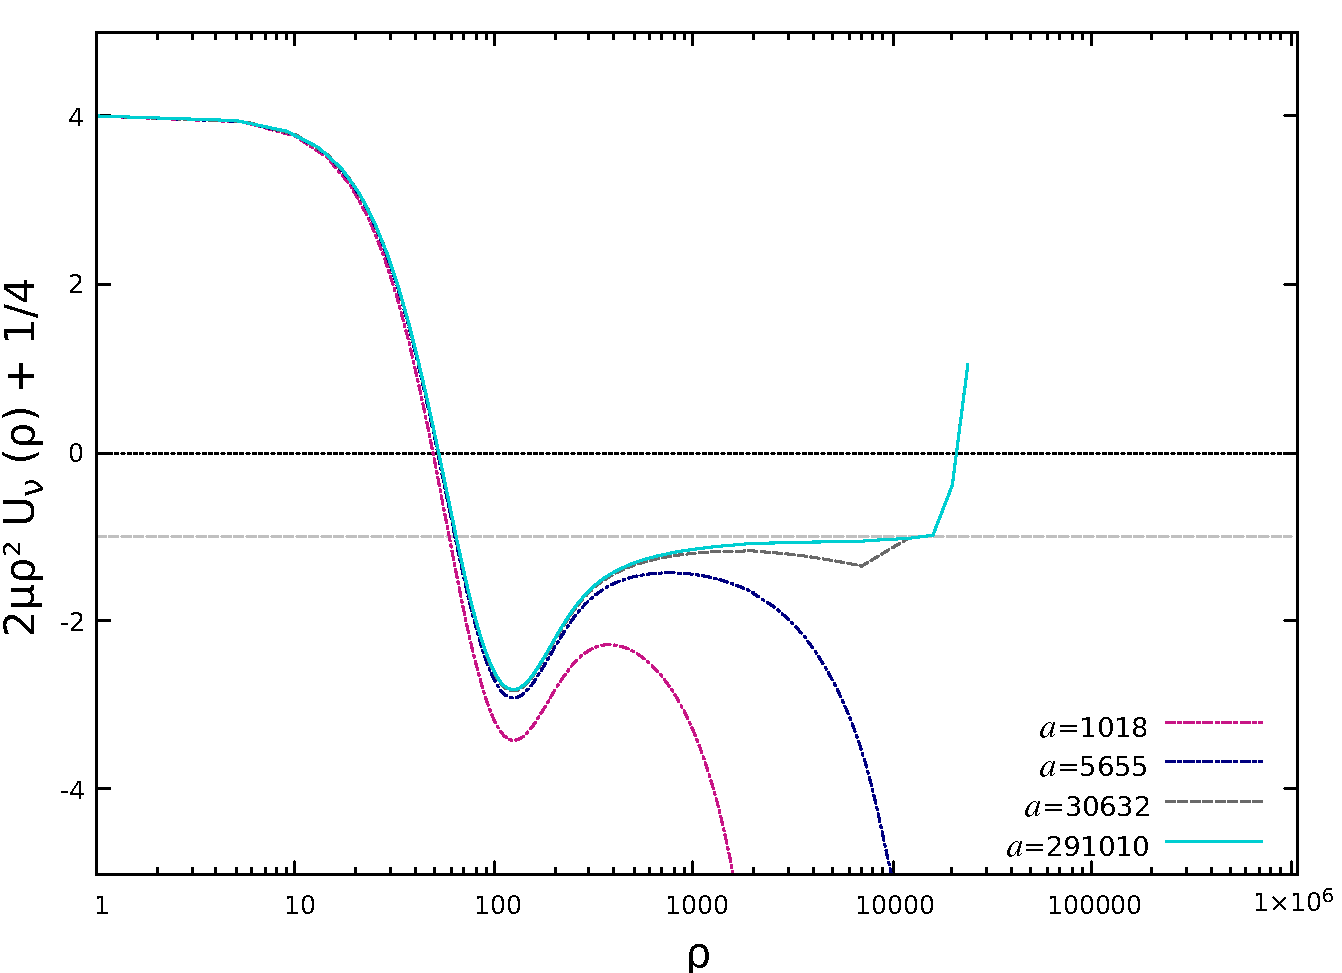
\includegraphics[width=\linewidth]{positive_a.pdf}
	\caption{..}
	\label{fig:6}
\end{figure}